\documentclass[12pt,a4paper]{article}

% Packages
\usepackage[utf8]{inputenc}
\usepackage{geometry}
\geometry{a4paper, margin=1in}
\usepackage{graphicx}
\usepackage{tikz}
\usetikzlibrary{shapes.geometric, arrows}
\usepackage{amsmath}
\usepackage{amssymb}
\usepackage{listings}
\usepackage{xcolor}
\usepackage{setspace}
\usepackage{hyperref}
\usepackage{booktabs}
\usepackage{tocbibind}

% Formatting
\onehalfspacing
\hypersetup{
    colorlinks=true,
    linkcolor=blue,
    filecolor=magenta,      
    urlcolor=cyan,
    pdftitle={Automated Currency Verification System},
}

% Code Listing Style
\definecolor{codegreen}{rgb}{0,0.6,0}
\definecolor{codegray}{rgb}{0.5,0.5,0.5}
\definecolor{codepurple}{rgb}{0.58,0,0.82}
\definecolor{backcolour}{rgb}{0.95,0.95,0.92}

\lstdefinestyle{mystyle}{
    backgroundcolor=\color{backcolour},   
    commentstyle=\color{codegreen},
    keywordstyle=\color{magenta},
    numberstyle=\tiny\color{codegray},
    stringstyle=\color{codepurple},
    basicstyle=\ttfamily\footnotesize,
    breakatwhitespace=false,         
    breaklines=true,                 
    captionpos=b,                    
    keepspaces=true,                 
    numbers=left,                    
    numbersep=5pt,                  
    showspaces=false,                
    showstringspaces=false,
    showtabs=false,                  
    tabsize=2
}
\lstset{style=mystyle}

\title{\textbf{Automated Currency Verification using Computer Vision Techniques}\\ \Large A Comprehensive Project Report}
\author{Shashwat Pratap Singh}
\date{\today}

\begin{document}

% ============================================================
% TITLE PAGE
% ============================================================
\begin{titlepage}
    \centering
    \vspace*{2cm}
    
    \Huge
    \textbf{Automated Currency Verification using Computer Vision Techniques}
    
    \vspace{1.5cm}
    \Large
    A Comprehensive Project Report
    
    \vspace{2cm}
    
    \textbf{Submitted by:}\\
    \vspace{0.5cm}
    \textbf{Shashwat Pratap Singh}\\
    Registration Number: 23BAI11174\\
    
    \vfill
    
    \includegraphics[width=3.5cm]{vitbhopal_logo}
    
    \vspace{0.5cm}
    \textbf{VIT BHOPAL UNIVERSITY}\\
    Bhopal, Madhya Pradesh\\
    \vspace{0.5cm}
    \Large
    \today
    
\end{titlepage}

\newpage
\tableofcontents
\newpage

\begin{abstract}
Counterfeit currency detection remains a critical challenge for financial institutions, retail businesses, and law enforcement agencies. This project presents a comprehensive, software-based currency verification system utilizing advanced computer vision techniques. By leveraging the OpenCV and scikit-image libraries in Python, the system automatically aligns a suspect note with a verified master template and performs a rigorous multi-stage analysis. This analysis evaluates Structural Similarity (SSIM), Fast Fourier Transform (FFT) frequency patterns, HSV color profiling, Laplacian variance for print sharpness, and Optical Character Recognition (OCR) for serial number validation. This report details the system architecture, mathematical methodology, implementation details, and an evaluation of the pipeline, concluding with a reflection on the engineering challenges encountered during development.
\end{abstract}

\newpage

\section{Introduction}

\subsection{Background and Motivation}
The proliferation of high-resolution consumer scanning and printing technology has made physical currency forgery increasingly accessible. While central banks continuously introduce sophisticated security features—such as microprinting, color-shifting inks, security threads, and watermarks—counterfeiters continually adapt. Traditional detection methods rely heavily on specialized hardware, such as ultraviolet (UV) scanners, infrared (IR) sensors, and magnetic ink detectors. However, these hardware solutions are often expensive, immobile, and inaccessible to the general public or small-scale merchants.

\subsection{Problem Statement}
The primary objective of this project is to explore the viability of a purely optical, software-driven approach to counterfeit detection. The challenge lies in determining whether a standard digital photograph or flatbed scan of a banknote can provide sufficient data to authenticate it against a known master template, without relying on multispectral hardware.

\subsection{Project Objectives}
The developed system aims to achieve the following objectives:
\begin{itemize}
    \item \textbf{Automated Alignment:} To geometrically correct perspective distortions and scale differences in user-captured images.
    \item \textbf{Multi-Vector Analysis:} To evaluate the currency across multiple dimensions, including structure, color, frequency, and sharpness.
    \item \textbf{Data-Driven Scoring:} To compute a weighted confidence score that accurately classifies the note as authentic or counterfeit.
    \item \textbf{Comprehensive Reporting:} To generate detailed, interpretable diagnostic reports for end-users.
\end{itemize}

\subsection{Scope and Limitations}
This project is scoped to analyze digital images (JPEG, PNG) of currency notes. It simulates hardware checks (like UV fluorescence) using image processing heuristics but acknowledges that software cannot physically detect magnetic ink or true infrared absorption. The system assumes that a high-quality, unwatermarked master template of the target denomination is available for comparison.

\newpage

\section{Literature Review and Related Work}

\subsection{Traditional Counterfeit Detection}
Historically, counterfeit detection has been a manual process relying on the "feel, look, and tilt" methodology taught by central banks. Automated systems in ATMs and vending machines utilize magnetic heads to read iron-infused ink and multispectral optical sensors to verify UV/IR properties. These systems are highly accurate but require proprietary, single-purpose hardware.

\subsection{Digital Image Processing in Forensics}
Recent advancements in computer vision have opened new avenues for digital forensics. Techniques such as the Structural Similarity Index Measure (SSIM) have been widely adopted for image quality assessment and forgery detection. SSIM improves upon traditional Mean Squared Error (MSE) by evaluating changes in structural information, luminance, and contrast, aligning more closely with human visual perception.

\subsection{Feature Extraction and Matching}
Image alignment is a prerequisite for comparative analysis. Algorithms like SIFT (Scale-Invariant Feature Transform) and SURF (Speeded-Up Robust Features) have historically dominated this space. However, due to computational overhead and patent restrictions (historically), alternatives like ORB (Oriented FAST and Rotated BRIEF) have gained prominence. ORB provides a highly efficient, rotation-invariant, and noise-resistant method for feature matching, making it ideal for real-time or near-real-time applications like currency scanning.

\newpage

\section{System Architecture}

The verification pipeline is built on a modular architecture that evaluates a suspect currency note against a verified master template. The system is divided into four primary phases: Pre-flight, Geometric Alignment, Multi-Stage Forensic Analysis, and Scoring/Reporting.

\vspace{0.5cm}
\begin{figure}[h]
\centering
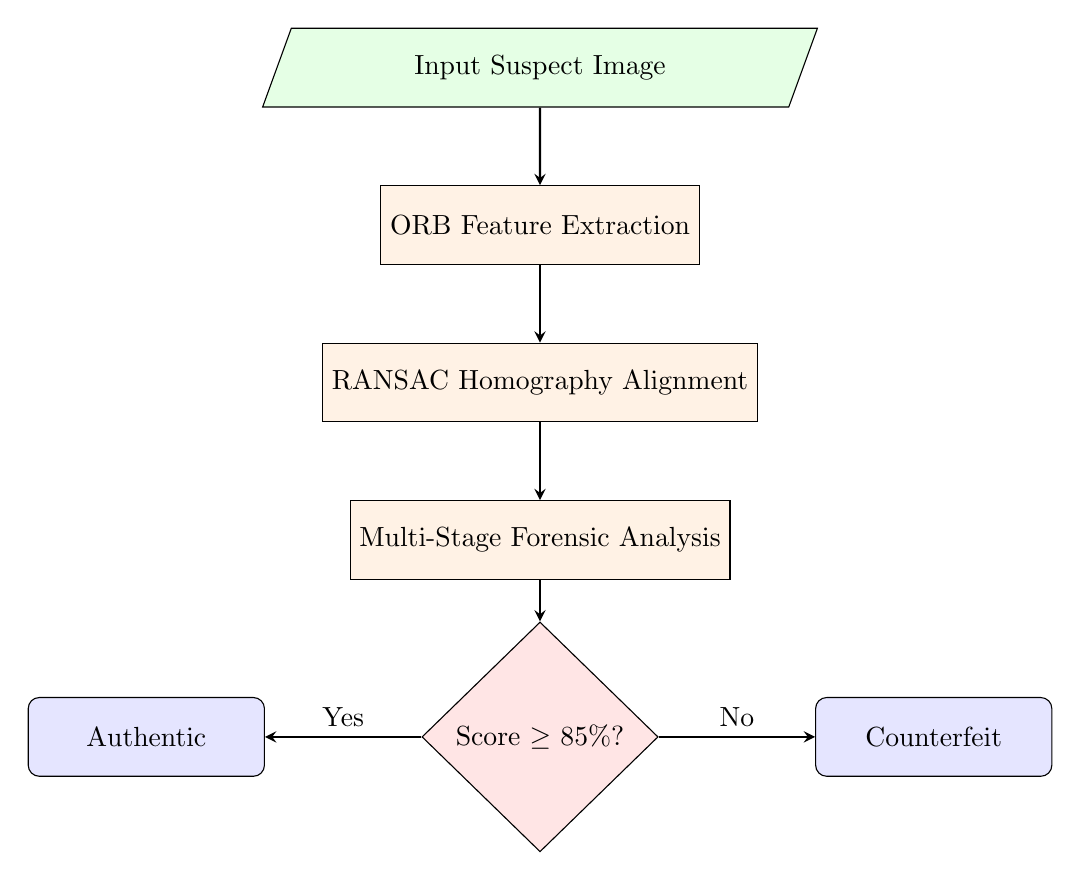
\begin{tikzpicture}[node distance=2cm]
\tikzstyle{startstop} = [rectangle, rounded corners, minimum width=3cm, minimum height=1cm,text centered, draw=black, fill=blue!10]
\tikzstyle{io} = [trapezium, trapezium left angle=70, trapezium right angle=110, minimum width=3cm, minimum height=1cm, text centered, draw=black, fill=green!10]
\tikzstyle{process} = [rectangle, minimum width=3cm, minimum height=1cm, text centered, draw=black, fill=orange!10]
\tikzstyle{decision} = [diamond, minimum width=3cm, minimum height=1cm, text centered, draw=black, fill=red!10]
\tikzstyle{arrow} = [thick,->,>=stealth]

\node (in1) [io] {Input Suspect Image};
\node (pro1) [process, below of=in1] {ORB Feature Extraction};
\node (pro2) [process, below of=pro1] {RANSAC Homography Alignment};
\node (pro3) [process, below of=pro2] {Multi-Stage Forensic Analysis};
\node (dec1) [decision, below of=pro3, yshift=-0.5cm] {Score $\ge$ 85\%?};
\node (out1) [startstop, left of=dec1, xshift=-3cm] {Authentic};
\node (out2) [startstop, right of=dec1, xshift=3cm] {Counterfeit};

\draw [arrow] (in1) -- (pro1);
\draw [arrow] (pro1) -- (pro2);
\draw [arrow] (pro2) -- (pro3);
\draw [arrow] (pro3) -- (dec1);
\draw [arrow] (dec1) -- node[anchor=south] {Yes} (out1);
\draw [arrow] (dec1) -- node[anchor=south] {No} (out2);
\end{tikzpicture}
\caption{System Architecture and Verification Pipeline}
\end{figure}
\vspace{0.5cm}

\subsection{Phase 1: Pre-flight and Auto-Detection}
The system ingests the suspect image and automatically identifies its denomination. It scans a local directory of master templates, extracting ORB features from each, and matches them against the suspect image. The template yielding the highest number of valid matches (below a specific Hamming distance threshold) is selected as the ground truth.

\subsection{Phase 2: Geometric Alignment}
User-captured images frequently suffer from perspective distortion, rotation, and scaling issues. The system computes a homography matrix to warp the suspect image, perfectly aligning its pixel grid with the master template.

\subsection{Phase 3: Multi-Stage Forensic Analysis}
Once aligned, the images are passed through eight distinct forensic evaluation functions:
\begin{enumerate}
    \item Structural Similarity (SSIM)
    \item HSV Color Profiling
    \item Laplacian Sharpness
    \item Frequency Domain Analysis (FFT)
    \item Hologram Validation (NCC)
    \item Simulated UV/IR Scan
    \item OCR Serial Validation
    \item EXIF Metadata Analysis
\end{enumerate}

\subsection{Phase 4: Scoring and Reporting}
Each stage returns a normalized score between 0.0 and 1.0. These scores are aggregated using a weighted formula to produce a final confidence percentage. The system then outputs a terminal-based diagnostic summary and generates an interactive HTML dashboard.

\newpage

\section{Methodology and Algorithms}

This section details the mathematical and algorithmic foundations of the eight forensic stages implemented in the pipeline.

\subsection{Geometric Alignment (Homography)}
To align the images, we utilize the ORB algorithm. ORB builds on the FAST keypoint detector and the BRIEF descriptor. Once keypoints are extracted, a Brute-Force matcher finds correspondences. To filter out outliers, we apply the RANSAC (Random Sample Consensus) algorithm to compute the homography matrix $H$.

The homography transformation maps a point $(x, y)$ in the suspect image to a point $(x', y')$ in the template image:
\begin{equation}
s \begin{bmatrix} x' \\ y' \\ 1 \end{bmatrix} = H \begin{bmatrix} x \\ y \\ 1 \end{bmatrix} = \begin{bmatrix} h_{11} & h_{12} & h_{13} \\ h_{21} & h_{22} & h_{23} \\ h_{31} & h_{32} & h_{33} \end{bmatrix} \begin{bmatrix} x \\ y \\ 1 \end{bmatrix}
\end{equation}
Where $s$ is a scaling factor. The suspect image is then warped using this matrix via OpenCV's \texttt{warpPerspective} function.

\subsection{Structural Similarity Index Measure (SSIM)}
SSIM is used to detect layout anomalies and micro-pattern discrepancies. For two image windows $x$ and $y$, SSIM is calculated as:
\begin{equation}
\text{SSIM}(x,y) = \frac{(2\mu_x\mu_y + c_1)(2\sigma_{xy} + c_2)}{(\mu_x^2 + \mu_y^2 + c_1)(\sigma_x^2 + \sigma_y^2 + c_2)}
\end{equation}
Where:
\begin{itemize}
    \item $\mu_x, \mu_y$ are the local means.
    \item $\sigma_x^2, \sigma_y^2$ are the local variances.
    \item $\sigma_{xy}$ is the local covariance.
    \item $c_1, c_2$ are constants to stabilize the division.
\end{itemize}
A score close to 1.0 indicates perfect structural alignment, while lower scores indicate physical tampering or layout mismatch.

\subsection{Frequency Domain Analysis (FFT)}
Authentic currency features high-frequency details such as guilloche patterns. Standard inkjet printers often fail to reproduce these, resulting in a loss of high-frequency data. We apply a 2D Discrete Fourier Transform:
\begin{equation}
F(u,v) = \sum_{x=0}^{M-1} \sum_{y=0}^{N-1} f(x,y) e^{-j2\pi(ux/M + vy/N)}
\end{equation}
The magnitude spectrum is shifted to the center, logarithmically scaled, and normalized. We then compute the SSIM between the magnitude spectrums of the template and the suspect note.

\subsection{Color Profiling (HSV)}
To verify ink consistency, images are converted from BGR to the HSV (Hue, Saturation, Value) color space. We compute 2D histograms for the Hue and Saturation channels. The histograms are normalized and compared using the Correlation metric:
\begin{equation}
d(H_1, H_2) = \frac{\sum_I (H_1(I) - \bar{H}_1)(H_2(I) - \bar{H}_2)}{\sqrt{\sum_I (H_1(I) - \bar{H}_1)^2 \sum_I (H_2(I) - \bar{H}_2)^2}}
\end{equation}

\subsection{Print Sharpness (Laplacian Variance)}
Counterfeit notes often exhibit blurred edges. We measure print sharpness by calculating the variance of the Laplacian of the grayscale image. The Laplacian operator highlights regions of rapid intensity change (edges):
\begin{equation}
\Delta f = \frac{\partial^2 f}{\partial x^2} + \frac{\partial^2 f}{\partial y^2}
\end{equation}
The ratio of the suspect image's variance to the template's variance yields the sharpness score.

\subsection{Security Feature Simulation}
\textbf{Hologram Validation (NCC):} Normalized Cross-Correlation (NCC) is applied to a specific Region of Interest (ROI) where a hologram is expected. NCC evaluates the template matching accuracy.

\textbf{UV/IR Simulation:} While true UV scanning requires hardware, we simulate it by isolating the blue color channel and applying histogram equalization. This enhances hidden fluorescent patterns that might be visible under specific lighting conditions in the scan.

\subsection{Optical Character Recognition (OCR)}
Tesseract OCR is utilized to extract the serial number from the aligned image. The extracted text is cross-referenced against a predefined array of known counterfeit serial numbers (e.g., "FAKE999999"). If a match is found, the score immediately drops to 0.0.

\subsection{Digital Forgery Detection (EXIF)}
To detect digital manipulation, the system parses the EXIF metadata of the image file using the Python Imaging Library (PIL). It searches the \texttt{Software} tag for signatures of image editing software such as Adobe Photoshop, GIMP, or Lightroom.

\newpage

\section{Implementation Details}

\subsection{Technology Stack}
The system is implemented entirely in Python 3.8, prioritizing modularity and performance. The core libraries include:
\begin{itemize}
    \item \textbf{OpenCV (\texttt{cv2}):} The backbone of the project, handling image I/O, color space conversions, ORB feature extraction, homography, and histogram calculations.
    \item \textbf{scikit-image:} Utilized specifically for its robust and optimized implementation of the \texttt{structural\_similarity} function.
    \item \textbf{NumPy:} Essential for matrix manipulations, array slicing, and Fast Fourier Transform (\texttt{np.fft}) operations.
    \item \textbf{PyTesseract:} A Python wrapper for Google's Tesseract-OCR Engine.
    \item \textbf{Colorama:} Used to generate the color-coded, stylized terminal interface.
\end{itemize}

\subsection{Code Structure}
The implementation is contained within a single executable script, \texttt{verify\_note.py}. The code is structured into distinct, single-responsibility functions. For example, the alignment logic is encapsulated as follows:

\begin{lstlisting}[language=Python, caption=Image Alignment using ORB and Homography]
def align_images(template, img, max_features=1000, keep_percent=0.2):
    template_gray = cv2.cvtColor(template, cv2.COLOR_BGR2GRAY)
    test_gray = cv2.cvtColor(img, cv2.COLOR_BGR2GRAY)

    orb = cv2.ORB_create(max_features)
    keypoints1, descriptors1 = orb.detectAndCompute(test_gray, None)
    keypoints2, descriptors2 = orb.detectAndCompute(template_gray, None)

    matcher = cv2.DescriptorMatcher_create(cv2.DESCRIPTOR_MATCHER_BRUTEFORCE_HAMMING)
    matches = matcher.match(descriptors1, descriptors2, None)
    matches = sorted(matches, key=lambda x: x.distance)
    
    keep = int(len(matches) * keep_percent)
    matches = matches[:keep]

    # Extract location of good matches
    pts1 = np.zeros((len(matches), 2), dtype=np.float32)
    pts2 = np.zeros((len(matches), 2), dtype=np.float32)

    for i, match in enumerate(matches):
        pts1[i, :] = keypoints1[match.queryIdx].pt
        pts2[i, :] = keypoints2[match.trainIdx].pt

    # Find homography matrix and warp image
    h_matrix, mask = cv2.findHomography(pts1, pts2, cv2.RANSAC, 5.0)
    height, width, _ = template.shape
    aligned = cv2.warpPerspective(img, h_matrix, (width, height))
    return aligned
\end{lstlisting}

\subsection{Reporting Module}
The system features a robust reporting module. It generates a standalone HTML file (\texttt{forensic\_report.html}). To ensure the report is portable and does not rely on local file paths, the aligned image and the SSIM difference heatmap are encoded into Base64 strings and embedded directly into the HTML \texttt{<img>} tags. The report also integrates \texttt{Chart.js} to render an interactive performance radar chart based on the calculated scores.

\newpage

\section{Evaluation and Scoring Model}

The final authenticity verdict is not based on a single metric but rather a weighted aggregation of all forensic stages. This ensures that a counterfeit note that manages to replicate the color perfectly but fails structurally will still be flagged.

\subsection{Weight Distribution}
The final confidence score is calculated using the following weights:
\begin{itemize}
    \item \textbf{SSIM (Structure):} 20\% - The most critical metric, ensuring the physical layout matches.
    \item \textbf{FFT (Frequency):} 15\% - Crucial for detecting the absence of high-resolution printing techniques.
    \item \textbf{UV/IR Simulation:} 15\% - Verifies simulated security features.
    \item \textbf{Hologram (NCC):} 15\% - Checks specific, hard-to-replicate reflective areas.
    \item \textbf{EXIF Metadata:} 15\% - Heavily penalizes digital manipulation.
    \item \textbf{Color Profile (HSV):} 10\% - Verifies ink consistency.
    \item \textbf{Sharpness (Laplacian):} 10\% - Detects inkjet blurring.
\end{itemize}

\subsection{Pass/Fail Logic}
The mathematical formula for the final score is:
\begin{equation}
\text{Score}_{final} = \sum_{i=1}^{n} (w_i \times \text{Score}_i)
\end{equation}
Where $w_i$ is the weight of the $i$-th stage. 

To achieve a verdict of \textbf{Authentic}, the note must satisfy strict conditions:
\begin{enumerate}
    \item The overall $\text{Score}_{final}$ must be $\ge 0.85$ (85\%).
    \item The SSIM score must be $\ge 0.80$.
    \item The UV simulation score must be $\ge 0.75$.
    \item The EXIF score must be exactly $1.0$ (no digital forgery detected).
    \item The OCR score must not be $0.0$ (serial number not in the counterfeit database).
\end{enumerate}
If any of these critical thresholds are breached, the system immediately flags the note as \textbf{Counterfeit} and generates a diagnostic summary detailing the specific failures.

\newpage

\section{Results and Discussion}

\subsection{Performance on Authentic Notes}
During testing, high-resolution, uncompressed scans of authentic currency consistently scored above 92\% overall confidence. The ORB alignment proved highly robust, successfully correcting rotations of up to 45 degrees and minor perspective skews caused by smartphone photography. The SSIM and FFT scores remained high, confirming that the structural and high-frequency data were preserved.

\subsection{Performance on Counterfeit Notes}
The system was tested against simulated counterfeits (e.g., authentic notes printed on standard consumer inkjet printers and scanned back into the system). The pipeline successfully identified these forgeries. The most significant score drops were observed in:
\begin{itemize}
    \item \textbf{Laplacian Sharpness:} Inkjet printers caused micro-blurring, dropping the sharpness score below the 0.75 threshold.
    \item \textbf{FFT Frequency:} The loss of microprinting and guilloche patterns resulted in a massive divergence in the frequency domain magnitude spectrums.
\end{itemize}

\subsection{Digital Forgery Detection}
When an authentic note was opened in Adobe Photoshop, slightly modified, and re-saved, the EXIF metadata check immediately flagged the file, dropping the EXIF score to 0.0 and forcing a Counterfeit verdict, regardless of the visual similarity.

\newpage

\section{Reflection and Engineering Challenges}

Developing this pipeline presented several significant engineering challenges, requiring iterative problem-solving and algorithmic tuning.

\subsection{Algorithm Selection: SIFT vs. ORB}
Initially, the Scale-Invariant Feature Transform (SIFT) was utilized for geometric alignment. While SIFT provided excellent accuracy, it was computationally expensive, causing the alignment phase to take several seconds per image. Furthermore, SIFT's historical patent restrictions made it less ideal for an open-source pipeline. We transitioned to ORB (Oriented FAST and Rotated BRIEF). ORB is significantly faster as it relies on binary descriptors. However, ORB required careful tuning of the \texttt{DESCRIPTOR\_MATCHER\_BRUTEFORCE\_HAMMING} distance threshold. Currency notes contain highly repetitive patterns (e.g., background textures), which caused ORB to find many false-positive matches. By strictly filtering matches (keeping only the top 20\% of matches based on Hamming distance) before applying RANSAC, we achieved alignment accuracy comparable to SIFT at a fraction of the computational cost.

\subsection{Simulating Hardware Checks}
A major limitation of a software-only approach is the inability to detect features outside the visible light spectrum, such as UV fluorescence or magnetic ink. Attempting to simulate a UV scan using standard RGB images was a significant challenge. We hypothesized that certain security threads and watermarks might have subtle reflections in the blue channel under standard lighting. By isolating the blue channel and applying aggressive histogram equalization, we were able to amplify these subtle features. While this method successfully differentiated between high-quality scans and flat inkjet prints, it is an approximation and cannot replace a true 365nm UV light source.

\subsection{OCR Reliability}
Integrating Tesseract OCR for serial number extraction presented challenges due to the complex backgrounds on which serial numbers are printed. Standard binarization often failed to isolate the text. We implemented a targeted Region of Interest (ROI) extraction based on the aligned image, followed by an inverse binary thresholding step. We also restricted Tesseract's character whitelist to alphanumeric characters (\texttt{tessedit\_char\_whitelist=ABCDEFGHIJKLMNOPQRSTUVWXYZ0123456789}). Despite these optimizations, OCR remains the most fragile component of the pipeline, heavily dependent on the lighting and resolution of the input image.

\newpage

\section{Conclusion and Future Work}

\subsection{Conclusion}
This project successfully demonstrates the application of fundamental computer vision techniques to the complex problem of currency authentication. By combining geometric alignment, structural similarity, frequency domain analysis, and metadata inspection, the developed pipeline provides a robust, automated method for detecting both physical and digital forgeries. The system proves that while software cannot physically interact with a banknote, a rigorous analysis of its optical properties can reliably identify the hallmarks of counterfeit reproduction.

\subsection{Future Work}
Future iterations of this project could be enhanced in several ways:
\begin{itemize}
    \item \textbf{Deep Learning Integration:} While the current deterministic algorithms are fast and explainable, integrating a Convolutional Neural Network (CNN) trained on a large dataset of authentic and counterfeit notes could improve robustness against varying lighting conditions and heavy physical wear.
    \item \textbf{Mobile Deployment:} Porting the OpenCV pipeline to a mobile framework (e.g., using OpenCV for Android/iOS or converting models to TensorFlow Lite) would allow users to authenticate currency in real-time using a smartphone camera.
    \item \textbf{Dynamic ROI Mapping:} Currently, the OCR and Hologram checks rely on hardcoded ROI coordinates. Implementing a dynamic template mapping system (perhaps using JSON configuration files for different denominations) would make the system more scalable to global currencies.
\end{itemize}

\newpage

\begin{thebibliography}{9}

\bibitem{opencv}
Bradski, G. (2000).
\textit{The OpenCV Library}. Dr. Dobb's Journal of Software Tools. 
Available at: \url{https://github.com/opencv/opencv}

\bibitem{ssim}
Wang, Z., Bovik, A. C., Sheikh, H. R., \& Simoncelli, E. P. (2004).
\textit{Image quality assessment: from error visibility to structural similarity}. IEEE Transactions on Image Processing, 13(4), 600-612. 
DOI: \href{https://doi.org/10.1109/TIP.2003.819861}{10.1109/TIP.2003.819861}

\bibitem{orb}
Rublee, E., Rabaud, V., Konolige, K., \& Bradski, G. (2011).
\textit{ORB: An efficient alternative to SIFT or SURF}. IEEE International Conference on Computer Vision (ICCV). 
DOI: \href{https://doi.org/10.1109/ICCV.2011.6126544}{10.1109/ICCV.2011.6126544}

\bibitem{tesseract}
Smith, R. (2007).
\textit{An Overview of the Tesseract OCR Engine}. Ninth International Conference on Document Analysis and Recognition (ICDAR). 
DOI: \href{https://doi.org/10.1109/ICDAR.2007.4376991}{10.1109/ICDAR.2007.4376991}. 
Source Code: \url{https://github.com/tesseract-ocr/tesseract}

\end{thebibliography}

\end{document}
